\section*{Bibliographie}
\subsubsection{Images utilisées}\label{images}
Les images utilisées sont des ressources qui m'ont été fournies par des employés au sein de l'entreprise ou des diagrammes que j'ai confectionnné lors de mon stage en entreprise.

\subsubsection{ISO/IEC 27001-2022}\label{iso}
Systèmes de management de la sécurité de l'information - Exigences\par
Édition en vigueur : ISO/IEC 27001:2022\par
État actuel : Publiée (stade 60.60)\par
Auteur : 
\begin{itemize}
    \item International Organization for Standardization (ISO)
    \item International Electrotechnical Commission (IEC)
\end{itemize}\par
Date de publication : 2022-10\par
Sources : 
\begin{enumerate}
    \item \href{https://www.cssia.org/wp-content/uploads/2020/01/ISO_27001_Standard.pdf}{\textcolor{imtneCeleste}{Liste de vérification des exigences de la norme ISO 27001 - [Lien vers le PDF]}}
    \item \href{http://www.itref.ir/uploads/editor/2ef522.pdf}{\textcolor{imtneCeleste}{Description détaillée des éléments de la norme ISO 27001 - [Lien vers le PDF]}}
\end{enumerate}






\newpage
\section*{Annexes}
\subsection*{Infrastructure de l'entreprise}
\begin{figure}[ht!]
    \centering
    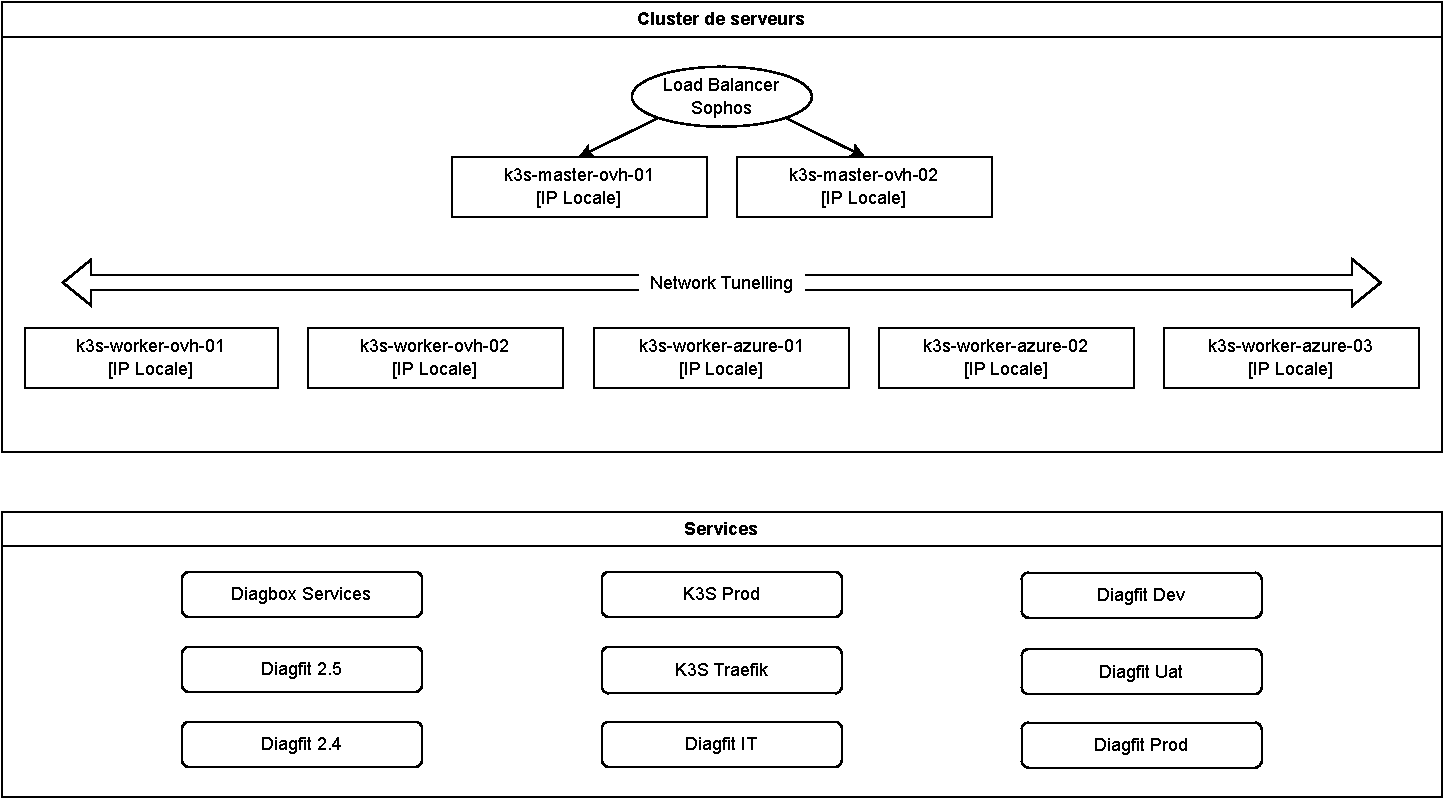
\includegraphics[width=\textwidth]{paper/figures/balancer.pdf}
    \label{balancer}
    \caption{Répartission de la charge de travail entre les différents serveurs}
\end{figure}

\clearpage
\newgeometry{top=0pt, bottom=0pt, inner=0pt, outer=0pt}
\thispagestyle{empty} % Pas de header, footer ou numéro de page
\begin{figure}[ht!]
    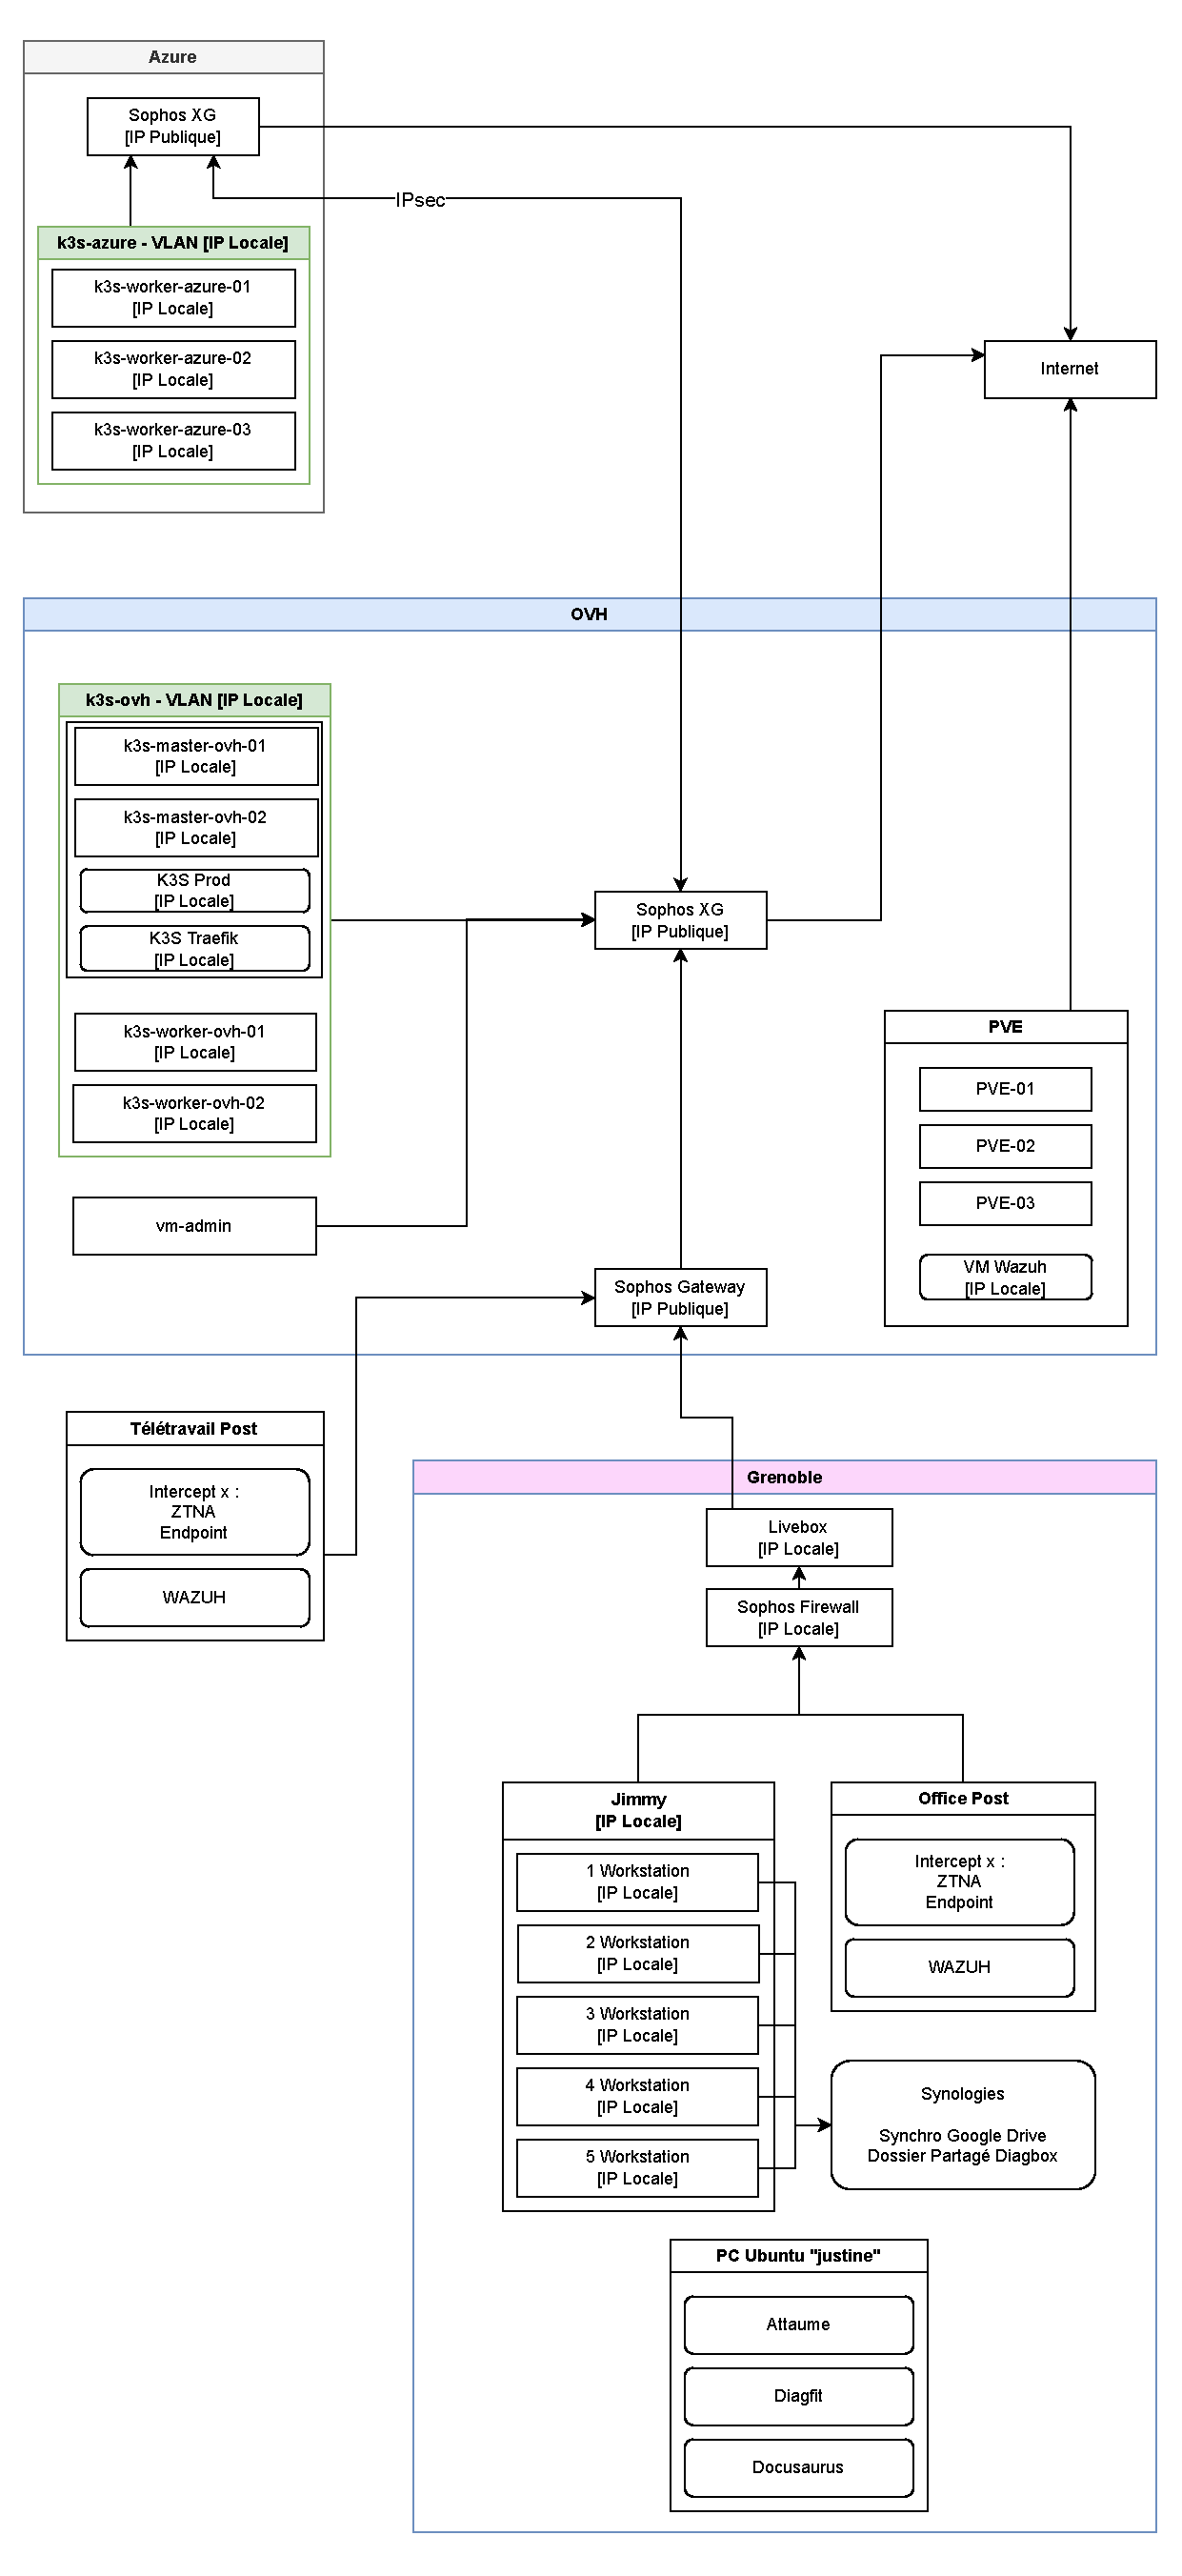
\includepdf{paper/figures/infra.pdf}
    \label{infra}
    \caption{Infrastructure}
\end{figure}
\restoregeometry % Rétablir la géométrie par défaut
\pagestyle{fancy}